%   Filename    : chapter_3.tex
\chapter{Research Methodology}

The steps outlined in the following sections were conducted.

\section{Data Gathering}

Filipino language news articles, both fake and authentic, were sourced from the internet.

Specifically, the data-gathering methodology outlined in the work of \cite{cruz2020localization} was adapted to refrain from reinventing the wheel and to ensure consistency between fresh and old data. To augment the Fake News Filipino dataset from their study with a similar dataset, fake news articles were sourced via web scraping from various fraudulent websites tagged by VERA Files. As an independent non-profit organization in the Philippines, its mission is to engage in extensive research and the writing and production of media, in pursuit of excellent journalism \cite{verafiles-about}. VERA Files has several fact-checking ventures, which include VERA Files Fact Check \cite{verafiles-fact-check}. On the other hand, authentic news articles were sourced from trusted mainstream providers such as The Philippine Star and ABS-CBN. Python's \textit{BeautifulSoup4} and \textit{selenium} libraries were utilized in the development of the article scraper. The articles and the corpus were encoded in UTF-8. Minimal preprocessing of the text was conducted to preserve features such as misspelled words and incorrect punctuation. The news articles were mostly Filipino with a few words in the English vernacular. Scraped fake news and authentic news were labeled accordingly as Fake (0) or Real (1).

\section{Model Training and Data Processing}
\label{sec:ModelTraining}

Figure \ref{fig:Model} shows the steps in model training and data processing. The text inputs were tokenized, the features were extracted, and the models were trained using the extracted features.

The corpus was tokenized using a pre-trained BPE tokenizer from \citeA{cruz2020localization}. Linguistic features highlighted by \citeA{fernandez-2019} as well as \citeA{fayaz-2022} were used in training the models. Table \ref{tab::Features} describes the features to be extracted and specifies their predictors. These features include traditional or surface-based features such as word count, sentence count, and character count. These features were extracted via a library of Python scripts designed specifically for the extraction of Filipino linguistic features \cite{imperial-2020, imperial-2021}. Through the same library, syllabic features based on the prescribed Philippine orthography, lexical features such as type-token ratio, and morphological features such as morphemes were extracted. Additionally, the misspelled word frequency, out-of-vocabulary (OOV) word frequency, stop word frequency, and the readability formula for modern Filipino texts developed by \citeA{Macahilig2015ACR}, which has not been investigated as a linguistic feature of Filipino texts in previous studies, were appended to the feature space. The tokens were vectorized with TF-IDF, extracting unigrams, bigrams, and trigrams as well as bag-of-words. The following classifiers were trained using the extracted features: Multinomial Naive Bayes, Logistic Regression, Random Forest, and Support Vector Classifier (SVC).

\begin{figure}[h]
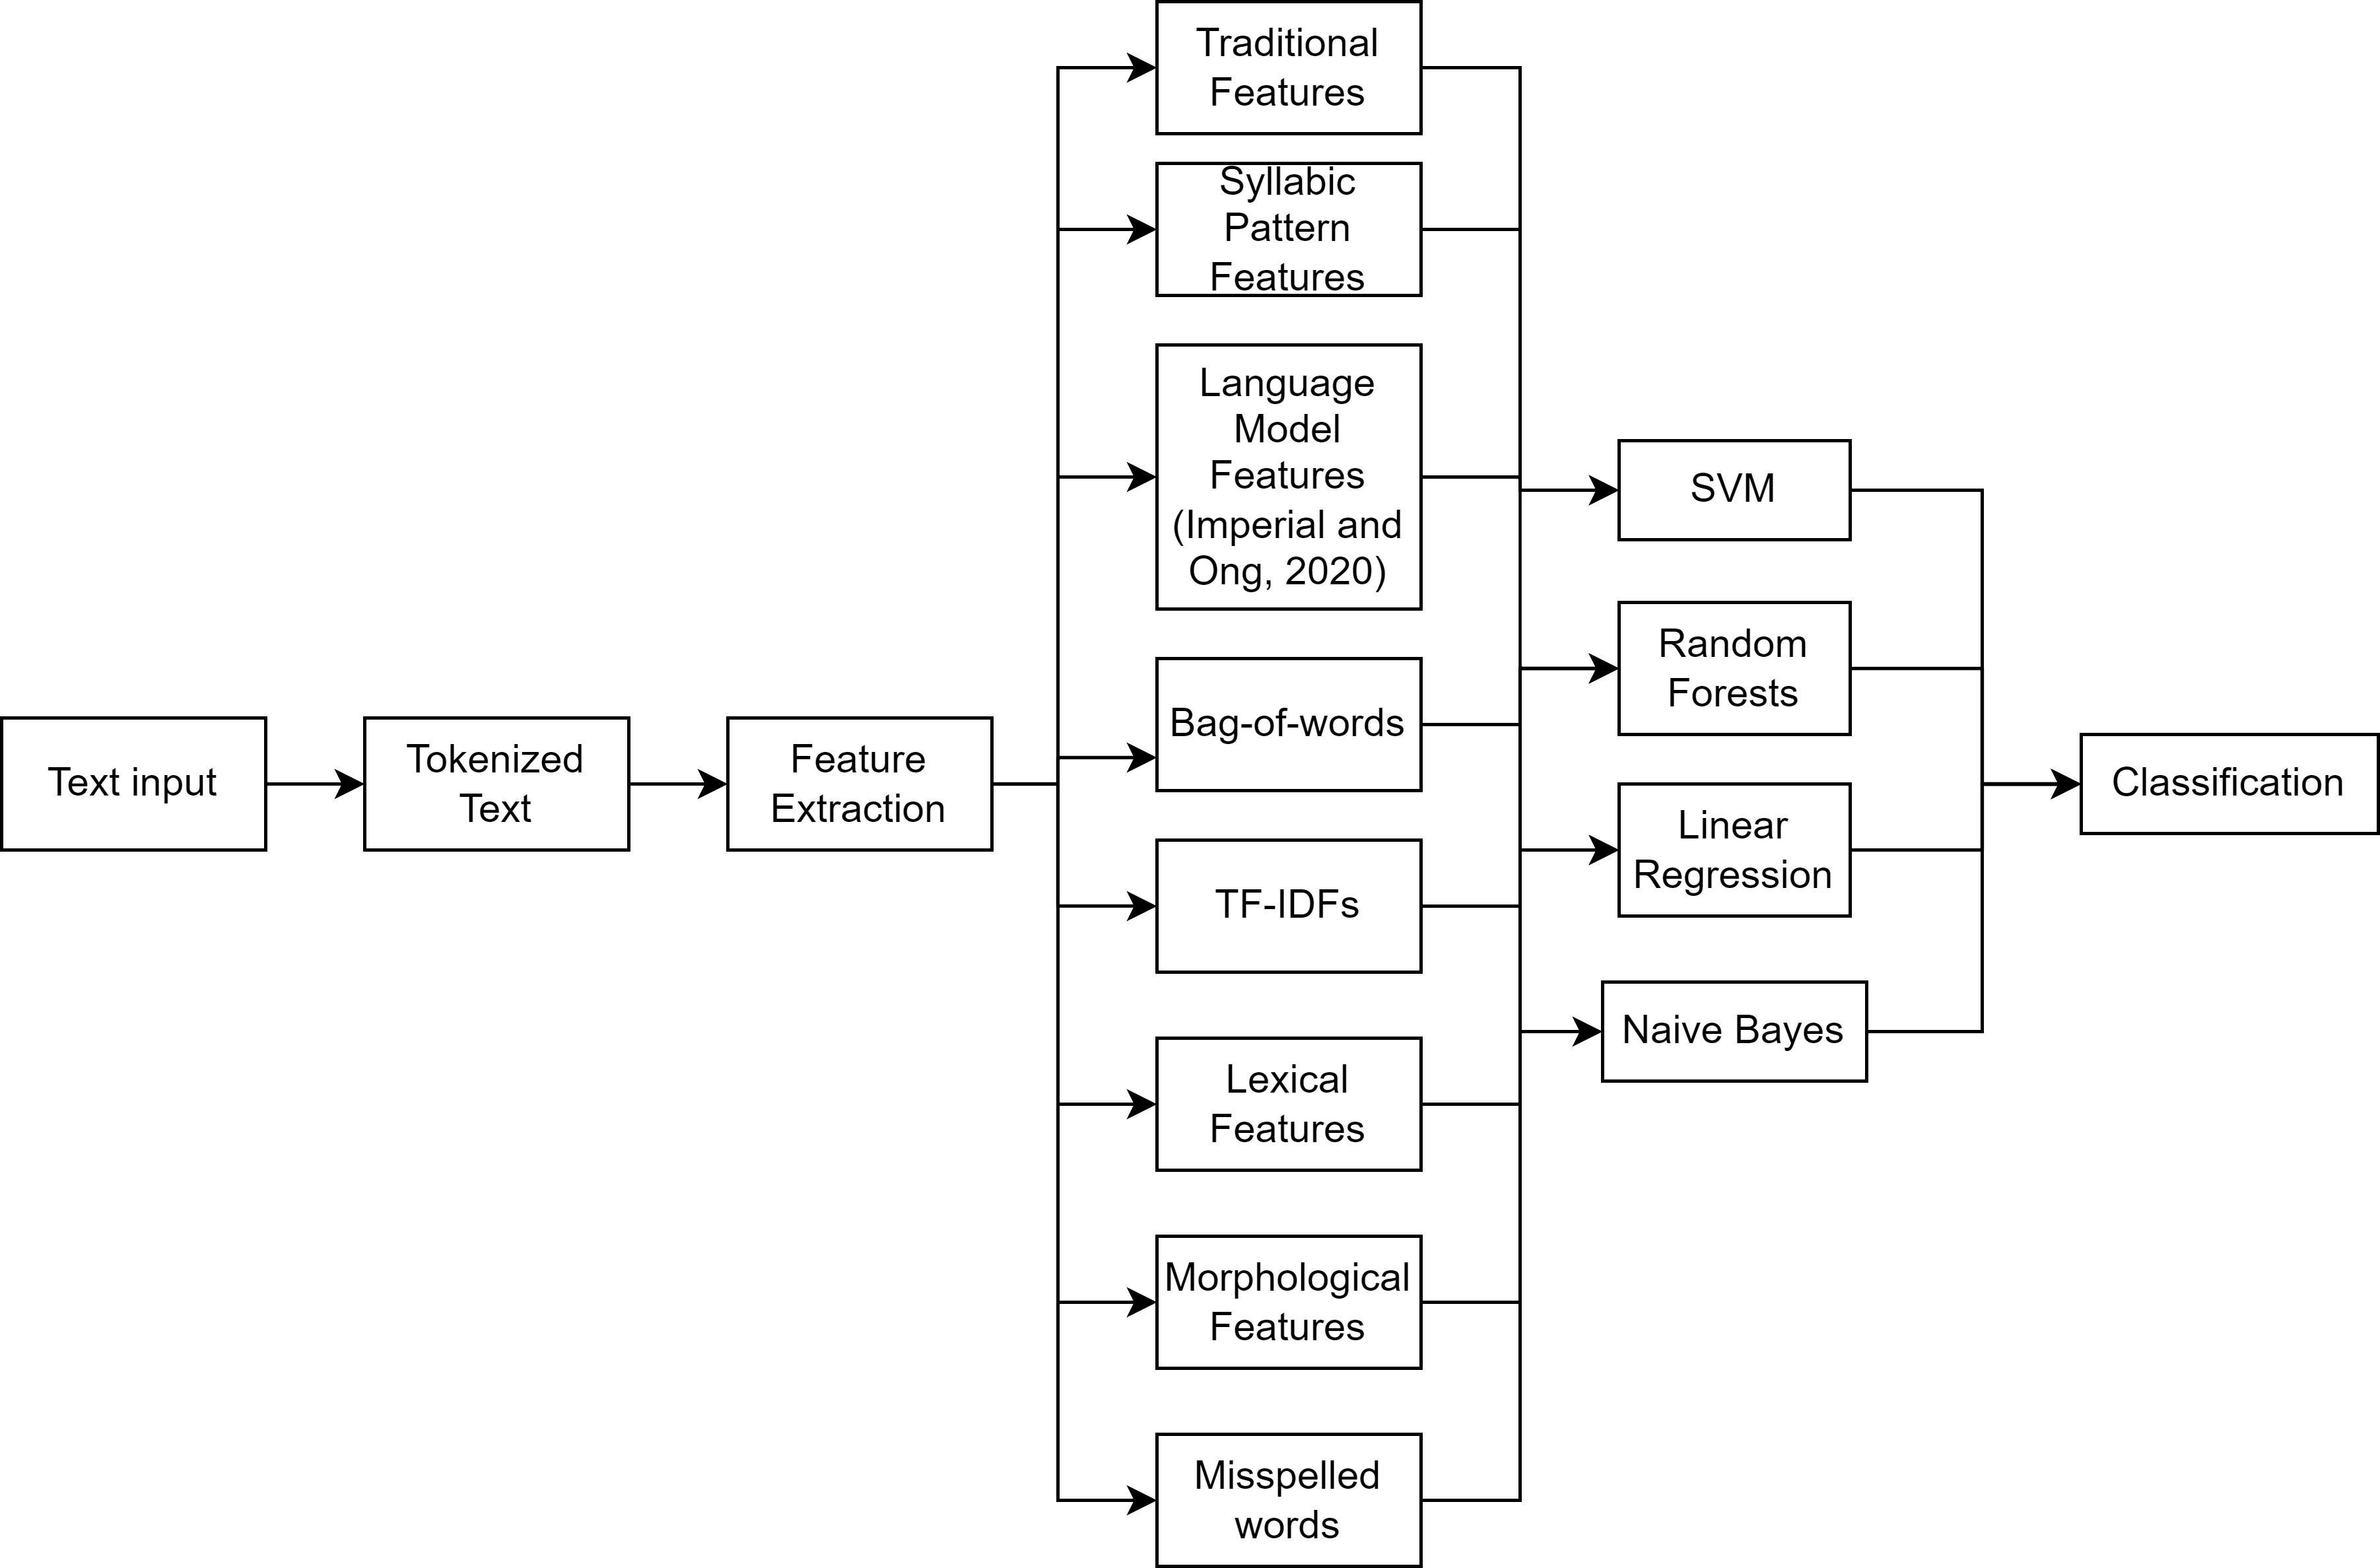
\includegraphics[width=\textwidth,height=\textheight,keepaspectratio]{figures/Model Training.png}
  \caption{Data Processing and Model Training}
  \label{fig:Model}
\end{figure}

\clearpage
\singlespacing
\begingroup
  \fontsize{10pt}{12pt}\selectfont
    \tablefirsthead{\hline Feature & Description & Predictors \\ \hline}
    \tablehead{
      \hline
      \multicolumn{3}{r}{Continued from previous column...} \\ \hline
      Feature & Description & Predictors \\ \hline
    }
    \tabletail{
      \hline \multicolumn{3}{r}{Continued in the next column...} \\ \hline
    }
    \tablelasttail{\\ \hline}
    \bottomcaption{Descriptions and predictors of features.}
    \label{tab::Features}
    \begin{xtabular}{|p{0.20\linewidth}|p{0.35\linewidth}|p{0.35\linewidth}|}
      Bag-of-words & Unordered collection of words. & Bag-of-words model of the input text. \\
      \hline
      TF-IDF & Word to document ratio in the corpus. & TF-IDF using \textit{n}-gram values of \{ 1, 2, 3\}. \\
      \hline
      Misspelled words & Misspelled words in the input text. & Total misspelled word count. \\
      \hline

      OOV words & Words in the input text that are not found in the Filipino and English dictionary used in training & Total OOV word count. \\
      \hline
      Stop words & words considered insignificant in processing text input e.g. "at", "ay", "din", etc. in Filipino or "a", "the", "to", "as" in English. & Total stop word count. \\
      \hline
      Filipino readability formula & Readability formula for Filipino text by \citeA{Macahilig2015ACR}. The higher the readability index, the more difficult the text is to read. & Readability is computed by: \( P = -4.161 + 0.280(w/s) + 0.106(cw)\) where P is the readability index, w/s is the average number of words per sentence, and cw is the word count. \\
      \hline
      Traditional & Traditional or Surface-based features based on counts and frequencies & Total word, sentence, phrase, polysyllabic word counts. Average word length, sentence length, syllable per word. \\
      \hline
      Syllabic Pattern & Syllable pattern densities based on the prescribed Philippine orthography & Prescribed Philippine orthography \{v, cv, vc, cvc, vcc, cvcc, ccvc, ccvcc, ccvccc\}, where c and v are consonant and vowel notations. \\
      \hline
      Lexical & Lexical or context-carrying features using part-of-speech categories. & Type-token variations (regular, logarithmic, corrected, root). Noun and verb token ratio. Lexical density. Foreign word and compound word density.\\
      \hline
      Morphological & Morphological features based on verb inflection. & Densities of foci of verbs based on tense: \{actor, object, benefactive, locative, instrumental, referential\}. Densities of various foci of verbs based on aspect: \{infinitive, perfective, imperfective, contemplative, participle, recent-past, auxiliary\}.
    \end{xtabular}
\endgroup
\doublespacing
\clearpage

To determine the optimal hyperparameters for the classifiers, grid search was used for hyperparameter tuning. The classifiers were trained and tested on the combined dataset using five-fold cross validation. The results of hyperparameter tuning were then used in the final training and testing of the models which involved using five-fold cross validation six times, which totals 30 trainings and testings.

For the analysis of accuracies, the Shapiro-Wilk test was first conducted to assess the normality of the data. Levene's test was then used to assess the homoscedasticity of the variances. Then, since there were two factors—the dataset and the classifier—two-way ANOVA for trimmed means was employed on the values to determine which classifiers had significant differences in which dataset, and to determine whether the accuracy of the classifier depends on the dataset. Post-hoc tests using Bonferroni correction was further performed for significant ANOVA results. 

\section{System Deployment}

\subsection{System Architecture}

The FaKe application system consisted of three components: a machine learning model deployed as a microservice, an application programming interface (API) running via a cloud server infrastructure to host the model, and a cross-browser extension to interface with the API.

A cloud server infrastructure was utilized through Render (a platform as a service). Render was chosen because its free tier presented numerous advantages such as automated load balancing, a generous bandwidth and build time allocation, and integration with GitHub—changes may be deployed within a few seconds of pushing to a pipelined repository \cite{render-docs}. While Render at its free tier was not suitable for enterprise-scale production, it was suitable for rapid prototyping and deployment of full-stack web applications.

For the client, a browser extension deployed via Tampermonkey, a cross-browser extension manager, was utilized. Tampermonkey allowed users to enhance the functionality of web pages by injecting a script (written in JavaScript) into the page. Tampermonkey was chosen as it was one of the most popular browser extension managers available on mainstream web browsers (e.g. Google Chrome, Mozilla Firefox, Microsoft Edge, Safari, Opera, Next). It granted web developers the ability to write browser-independent code, and it provided a library of extensions to make them easy to deploy and install \cite{tampermonkey-website}.

Python was the programming language in the backend as it was the programming language of choice when it came to machine learning. It provided ease of compatibility between the API and the model. The API was built with FastAPI, a modern web framework for building RESTful APIs in Python. FastAPI was chosen because it had very high performance (one of the fastest Python web frameworks available, on par with NodeJS and Go). It was easy to use and had a smooth learning curve, and it complied with open standards for API (OpenAPI and JSON Schema) \cite{fastapi-website}.

\subsection{System Usage}

As Figure \ref{SystemFlowchart} shows, the user interacted with the FaKe browser extension while reading a Filipino language news article. A stable internet connection was required to establish communication between the FaKe browser extension and API.

The FaKe browser extension scraped the paragraph body of the article and packed it in a JSON. This packed JSON was sent to the API that hosted the machine learning model. The API unpacked the JSON and extracted Filipino linguistic features from the article text. The API employed exactly the same modules used in the extraction of Filipino linguistic features during model training. No sensitive information such as user credentials or IP addresses was transmitted. Once the Filipino linguistic features were extracted, the API used the model to make predictions on these features. The model identified whether the article was fake or not, entailing a waiting period of up to 30 seconds. The waiting period hinged on the state of the server and the length of the article. If an error during this exchange occurred, the user was notified and prompted to try again. However, if no error occurred and the model successfully predicted whether the article was fake or not, the API returned the prediction as a response JSON to the browser extension. The browser extension unpacked this response JSON and displayed the prediction (fake or real) to the user.

\begin{figure}[h]
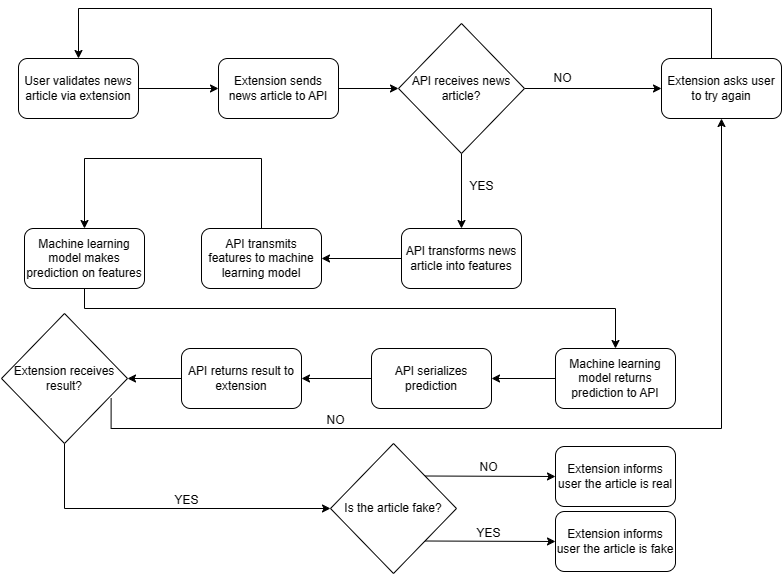
\includegraphics[width=\textwidth,height=\textheight,keepaspectratio]{figures/FakeSystemFlowchart.png}
  \caption{FaKe High Level System Flowchart}
  \label{SystemFlowchart}
\end{figure}
\clearpage

\subsection{System Limitations} \label{extension-limitations}

The FaKe API was hosted on a cloud server that spun down after long periods of inactivity. Free deployment instances at Render spun down after 15 minutes of no inbound traffic \cite{render-docs}, requiring time to spin back up. This meant that it took longer to respond to requests if no requests were sent for a long time. Once the server was active, requests may be promptly handled. Due to service and infrastructure constraints, models trained with morphological and lexical features, features that required a Java runtime to be extracted, were unable to be deployed over the web.

The FaKe browser extension as a tool only functioned reliably on news articles written in the Filipino language. Results from making predictions on news articles in English or other languages were unreliable at best. However, the FaKe browser extension had no way of limiting its usage to Filipino language news articles. Furthermore, predictions made by the FaKe browser extension may be inaccurate and may not reflect real-world events. Thus, the responsible usage of the FaKe browser extension rested with the user.

In this regard, we advocate for the hybrid approach in detecting fake news, wherein the employment of the FaKe browser extension is accompanied by dutiful and informed fact-checking. We make no claims that FaKe is a singular catch-all solution to detecting Filipino language fake news.